\section{azureml-core (Python SDK)}
% I want to be this guy, who builds with his team an increatiable A.I: system for munich.

\subsection{Connect to Workspace}
A workspace is a resource, which is tied (child) to a subscription and a resource group. A workspace links the different object to run a \gls{ML} model: Experiment, Training, Deployment. A workspace comes with a \gls{SDK} to interactive with.\\

To connect to the workspace, the constructor requires different parameters
\begin{lstlisting}[style=python]
	Workspace(
	subscription_id, resource_group, workspace_name,
	auth=None,
	_location=None,
	_disable_service_check=False,
	_workspace_id=None,
	sku='basic',tags=None, _cloud='AzureCloud'
	)
\end{lstlisting} 


\begin{comment}
\begin{figure}[H]
	\centering
	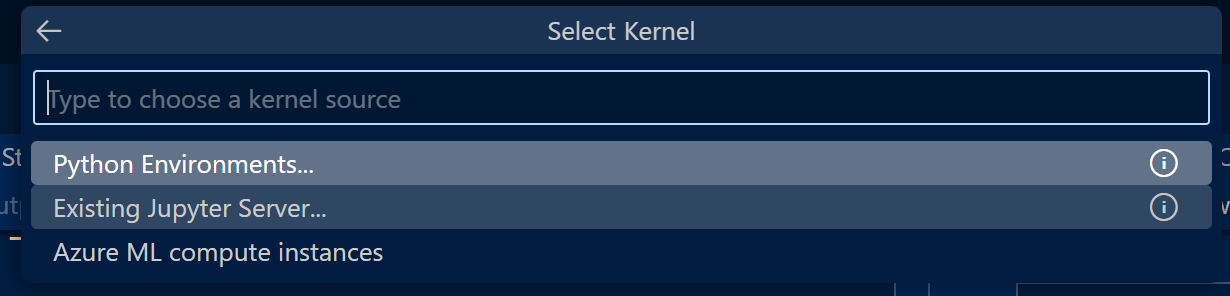
\includegraphics[scale = 0.3]{attachment/chapter_AML/Scc001}
	\caption{Connect to the workspace: Select kernel}
\end{figure}

We started, with writing the configuration file.
A started with opening jupter notebook and den selecting the kernel. And a kernel was installed on the compute cluster.
The authen

\\
auth
ServicePrincipalAuthentication or InteractiveLoginAuthentication or MsiAuthentication
default value: None
The authentication object. For more details, see https://aka.ms/aml-notebook-auth. If None, the default Azure CLI credentials will be used or the API will prompt for credentials.


\begin{lstlisting}[style=python]
	from azureml.core import Workspace
	ws = Workspace.create(name='myworkspace',
	subscription_id='<azure-subscription-id>',
	resource_group='myresourcegroup',
	create_resource_group=True,
	location='eastus2'
	)
	
	for i in range(n):
	print('i = ', i)
\end{lstlisting}


\end{comment}



